\chapter{Introducción}
\label{cap:introduccion}

\chapterquote{Los seres humanos no nacen para siempre el día en que sus madres los alumbran, sino que la vida los obliga a parirse a sí mismos una y otra vez}{Gabriel García Márquez}

\section{Motivación}
A lo largo de los años, los videojuegos han evolucionado considerablemente, llegando a convertirse en una parte muy importante del entretenimiento de hoy en día. Desde las sencillas primeras experiencias de las consolas hasta los complejos mundos actuales, los videojuegos han conquistado audiencias de todas las edades y culturas. A lo largo de esta evolución los enemigos han jugado un papel fundamental, haciendo que los videojuegos presentasen desafíos que atrapan a los jugadores. 
En el caso de los videojuegos 2D de plataformas, los enemigos son más que una simple oposición del jugador si no que son clave para mostrar la esencia del juego. El Pac-Man no sería lo mismo sin sus fantasmas ni el Super Mario sin sus Goombas. \\
Diseñar enemigos, especialmente en este tipo de juegos, es una tarea compleja. No solo trata de darles cierta apariencia si no que tienen que tener unos comportamientos y características únicas.  Esto implica que la persona encargada de esta tarea tiene que tener ciertos conocimientos en arte, diseño y programación. En la actualidad, este trabajo es realizado por personas de los campos anteriomente mencionados: artistas, diseñadores y programadores.
En los últimos años han surgido herramientas que simplifican significativamente el trabajo de los diseñadores, pero muy pocas están centradas específicamente en el diseño de enemigos. El objetivo de estas herramientas es el de facilitar el trabajo de los diseñadores para, incluso sin tener ni idea de programación, tener la capacidad de crear enemigos totalmente funcionales.


\section{Objetivos}
Este trabajo tiene como objetivo principal el diseño y desarrollo de un herramienta en C sharp para el motor de videojuegos Unity, que simplifique y agilice el proceso de creación de enemigos en juegos plataformas 2D. La herramienta contará con un catalogo de comportamientos fácil de manejar para cualquier persona independientemente de sus conocimientos de programación. El catálogo estará compuesto por tres categorías diferentes: acciones, sensores y eventos. Estos se definirán más adelante. \\
Para llevar a cabo el desarrollo de nuestra herramienta, vamos a documentarnos con herramientas similares y de como funcionan los enemigos en este tipo de juegos tomando como referencia títulos de renombre que serán presentados posteriormente.


\section{Plan de trabajo}
Para llevar a cabo este trabajo, se ha seguido la metodología ágil Scrum. Esta metodología, permite crear un flujo de trabajo enfocado en la iteración y continua mejora, asegurando un avance en el desarrollo eficiente y posibles adaptaciones frente a problemas detectados durante el proceso. 
El trabajo se dividirá en cuatro bloques: investigación y planificación, desarrollo de la memoria, desarrollo de la herramienta y pruebas con usuarios.
Cada bloque a su vez se dividirá en subsecciones explicadas a continuación.
\begin{itemize}
    \item  Investigación y planificación:
	\begin{itemize}
	    \item  Estudio del problema: En esta primera fase se realizará un estudio del estado del arte, centrado en el papel de los enemigos en los videojuegos, su importancia en la jugabilidad y las diferentes técnicas utilizadas para su diseño y comportamiento.
	    \item Selección y estudio de herramientas: Esta fase implicará un análisis comparativo de distintas técnicas y motores de videojuegos evaluando sus ventajas y desventajas, así como un estudio de su funcionamiento y  arquitecturas.
	    \item Diseño de la herramienta: En esta etapa, se definirá la arquitectura de la herramienta propuesta, describiendo las técnicas empleadas, esquemas de funcionamiento y organización de elementos principales.
	\end{itemize}
  \item Desarrollo de la memoria: 
	\begin{itemize}
	    \item  Redacción inicial: Es esta fase del trabajo se procederá a la redacción inicial de los contenidos cubriendo todos los puntos especificados en el índice.
	    \item Revisión y corrección: Una vez completada la redacción inicial, se realizarán las correcciones necesarias tras revisar exhaustivamente el documento.
	    \item Conclusiones y trabajo futuro: Tras finalizar los desarrollos y las pruebas de usuario, se redactarán las conclusiones obtenidas en base a los resultados y se detallarán los posibles pasos a seguir en un futuro.
	\end{itemize}
    \item Desarrollo de la herramienta: 
	\begin{itemize}
	    \item  Implementación de funcionalidades principales: En esta etapa se implementarán las funcionalidades principales de los movimientos básicos incluyendo la integración con sensores y emisores permitiendo la interacción entre ellos.
	    \item Implementación de ayuda visual: Se desarrollarán ayudas visuales destinadas a servir como referencias para los diseñadores, incluyendo elementos gráficos que faciliten la comprensión de los comportamientos. Además se implementará una herramienta que permita elegir y configurar de una forma más sencilla los componentes.
	    \item Pruebas y depuración: Se llevará a cabo un proceso iterativo de pruebas que aseguren la funcionalidad de la herramienta, corrigiendo los errores detectados durante su implementación.
	\end{itemize}
    \item Pruebas con usuarios:
	\begin{itemize}
	    \item Primera fase de pruebas: Se harán pruebas con usuarios que no hayan probado la herramienta antes, siguiendo un plan de pruebas especificado en el apartado "evaluación con usuarios". Las pruebas estarán centradas en: detectar posibles errores en las funcionalidades principales, validar la funcionalidad y evaluar la usabilidad y claridad.
	    \item Segunda fase de pruebas: Tras implementar mejoras recibidas del feedback de la primera prueba, se llevará a cabo una segunda prueba de verificación.
	    \item Corrección y resultados: Tras analizar los resultados de cada fase de prueba,se documentarán los errores y dificultades encontrados. Tras esto se procederá a implementar las correcciones necesarias para mejorar los resultados. 
	\end{itemize}
\begin{figure}[h]
	\centering
	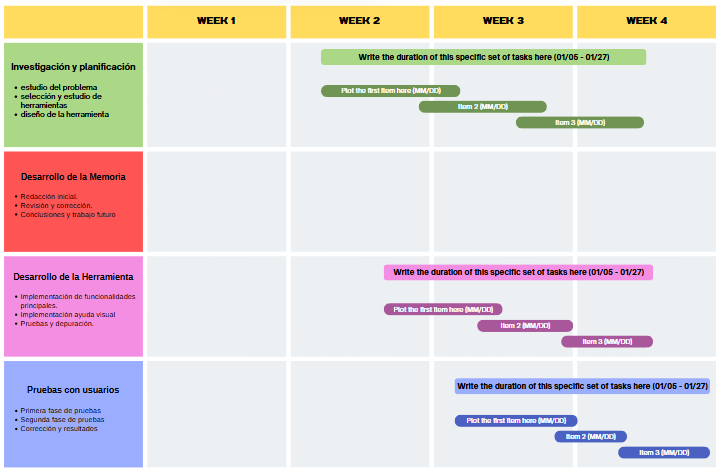
\includegraphics[width = 1\textwidth]{Imagenes/TabladeGantt.png}
	\caption{Tabla de Gantt }
	\label{fig:Tabla de Gantt}
\end{figure}
\end{itemize}
